\documentclass{article}

\usepackage[dvipsnames]{xcolor}
\usepackage{etoolbox}
\usepackage{hyperref}
\usepackage{minted}
\usemintedstyle{monokai}
\usepackage{titlesec}
\usepackage{setspace}
\usepackage[english]{babel}
\usepackage[a4paper, total={6in, 8in}]{geometry}
\usepackage{todonotes}
\usepackage[font={color=white},figurename=Fig.,labelfont={it}]{caption}
\usepackage{chngcntr}
\usepackage{titlecaps}
\usepackage{graphicx}
\usepackage{float}
\usepackage{wrapfig}
\usepackage{caption}
\usepackage{subcaption}
\usepackage[utf8]{inputenc}
\usepackage{fancyhdr}
\usepackage{lastpage}
\usepackage{todonotes}

\graphicspath{ {./images/} }

\hypersetup{colorlinks,
	linkcolor=white,
	linktoc=all}

\makeatletter % change only the display of \thepage, but not \thepage itself:
\patchcmd{\ps@plain}{\thepage}{\textcolor{white}{\thepage}}{}{}
\makeatother

\definecolor{bg}{HTML}{282828}
\colorlet{LightRubineRed}{RubineRed!70}
\colorlet{Mycolor1}{green!10!orange}
\definecolor{Mycolor2}{HTML}{00F9DE}

\setcounter{tocdepth}{3}

\renewcommand{\thesection}{\arabic{section}}

\renewcommand{\thepart}{
    \Alph{part}}

\title{Proj 2 Web Service \\ `Plantronixs' Plant Information System}
\author{Thomas Rhodes \\ 459274825}
\date{Last Updated: \today}

\begin{document}
    \pagestyle{fancy}
    \fancyhead[C]{}
    \fancyhead[LR]{}
    \fancyfoot[C]{\textcolor{white}{RHODES\_459274825\_PROJ2}}
    \fancyfoot[L]{\textcolor{white}{\thepage\ of \pageref{LastPage}}}
    \fancyfoot[R]{\textcolor{white}{Version: 1.0 \today}}
	\pagecolor{darkgray}
    \color{white}%
	
	\maketitle


	\tableofcontents
	\addtocontents{toc}{~\hfill\textbf{Page}\par}
	
	\newpage
	
	\begin{spacing}{2.5}
	\end{spacing}
    

    \part{Implementation}
    \begin{spacing}{4}
    \end{spacing}
	
	\section{Web Service That Supports at Least Four Unique Get and Post Actions}
	
	Post actions for this application can be seen when creating a new User, Plant, Family, Genus, PlantInfo, SoilPreference, UserPlant, Edible And when signing into the admin panel.
	
	\subsection{Terminal Outputs for Post Requests:}
	
	Admin Login Post Request
	\begin{minted}[bgcolor=bg]{console}
		[12/Apr/2022 23:22:23] "POST /admin/login/?next=/admin/ HTTP/1.1" 302 0
	\end{minted}
	\\
	api\_auth Login Post Request
	\begin{minted}[bgcolor=bg]{console}
		[12/Apr/2022 23:21:36] "POST /api-auth/login/ HTTP/1.1" 302 0
	\end{minted}
	\\
	Create User Post Request
	\begin{minted}[bgcolor=bg]{console}
		[12/Apr/2022 23:35:09] "POST /admin/auth/user/add/ HTTP/1.1" 200 7574
	\end{minted}
	\\
	Create genus Post Request
	\begin{minted}[bgcolor=bg]{console}
		[12/Apr/2022 23:44:00] "POST /genus/ HTTP/1.1" 201 9640
	\end{minted}
	\\
	Create Family Post Request
	\begin{minted}[bgcolor=bg]{console}
		[12/Apr/2022 23:48:22] "POST /family/ HTTP/1.1" 201 9671
	\end{minted}
	\\
	Create Plant Post Request
	\begin{minted}[bgcolor=bg]{console}
		[12/Apr/2022 23:51:30] "POST /plants/ HTTP/1.1" 201 11497
	\end{minted}
	\\
	Create PlantInfo Post Request
	\begin{minted}[bgcolor=bg]{console}
		[13/Apr/2022 00:08:37] "POST /info/ HTTP/1.1" 201 13509
	\end{minted}
	\\
	Create Soil Preference Post Request
	\begin{minted}[bgcolor=bg]{console}
		[13/Apr/2022 02:46:26] "POST /soilpreference/ HTTP/1.1" 201 11164
	\end{minted}
	\\
	Create User Plant Post Request
	\begin{minted}[bgcolor=bg]{console}
		[13/Apr/2022 02:47:48] "POST /userplant/ HTTP/1.1" 201 10234
	\end{minted}
	\\
	Create Edible Post Request
	\begin{minted}[bgcolor=bg]{console}
		[13/Apr/2022 02:48:34] "POST /edible/ HTTP/1.1" 201 13914
	\end{minted}
	
    
	\section{Build a correctly formed database to implement the \\specifications of Proj1} 
    
    \subsection{Defining the Database Tables}
    
    Screenshots below depict the code in `models.py' Which is used to define the database for this project, excluding the user, groups, permissions, and ip\_logging, tables which are created by Django and the ip\_logging middleware respectively:
    
    \begin{figure}
        \centering
        \caption{Models.py 1/4}
        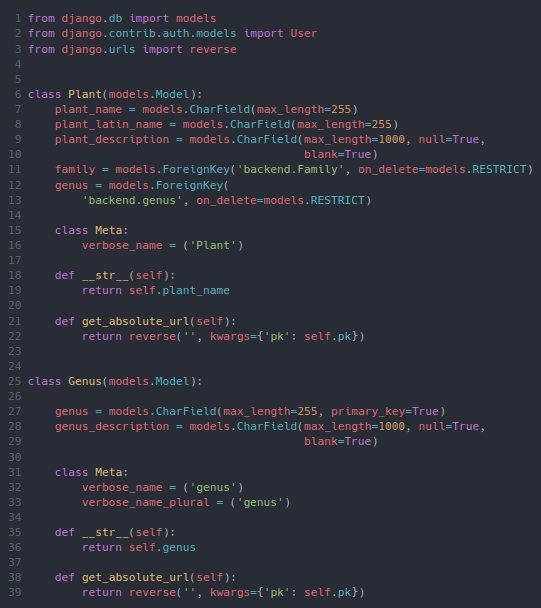
\includegraphics{models1}
    \end{figure}

    \begin{figure}
        \centering
        \caption{Models.py 2/4}
        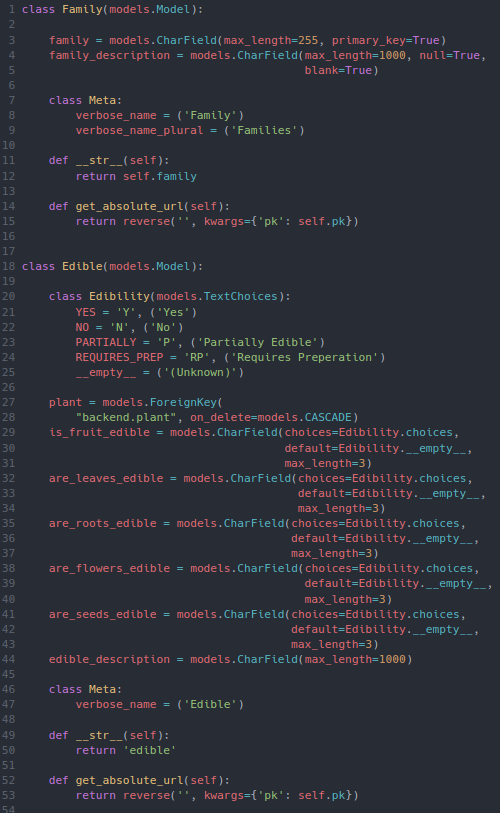
\includegraphics[scale=0.9]{models2}
    \end{figure}

    \begin{figure}
        \centering
        \caption{Models.py 3/4 Part 1}
        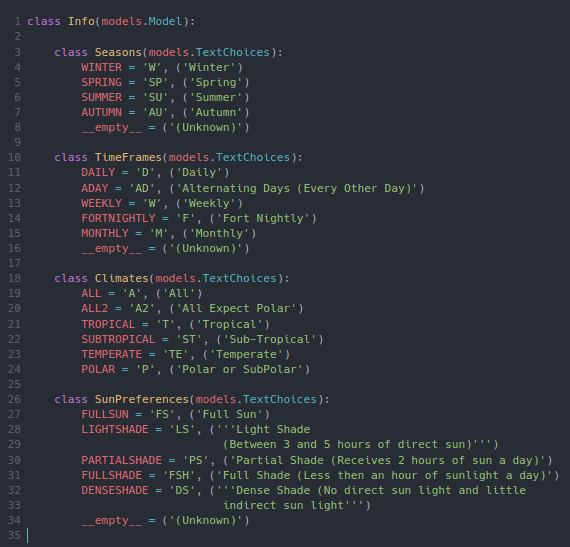
\includegraphics{models3-1}
    \end{figure}

    \begin{figure}
        \centering
        \caption{Models.py 3/4 Part 2}
        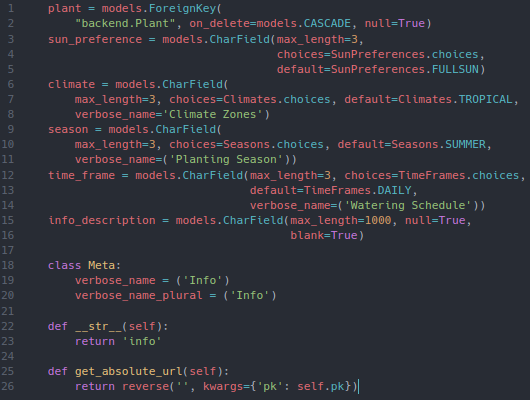
\includegraphics{models3-2}
    \end{figure}
    

    \begin{figure}
        \centering
        \caption{Models.py 4/4}
        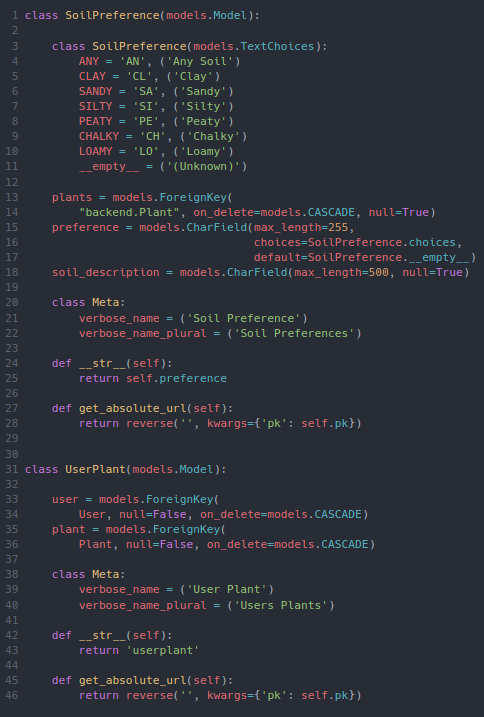
\includegraphics{models4}
    \end{figure}

    \newpage


    \subsection{Generated Database Tables}
    Using beekeeper studio, or with the use of the VSCode Extension `SQLite', we are able to see all of the generated tables in the database including, all which are automatically created by django. \\Screenshots provided below:

        \begin{figure}[!htb]
            \centering
            \caption{Table List and User\_Auth Table: \\ 8 of these tables are of relevancy to the specifications outlined in Proj1, These include auth\_user, backend\_edible, backend\_family, backend\_genus, backend\_info, backend\_plant, backend\_soilpreference, backend\_userplant, as shown in the right image of Fig. 6, and Fig. 7, Fig. 8, and Fig. 9 Below}
            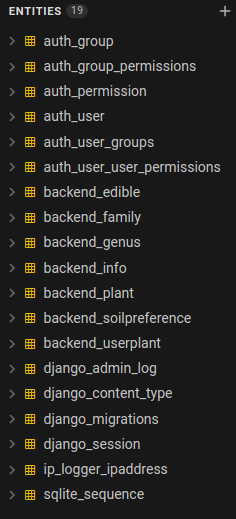
\includegraphics{sql1}
            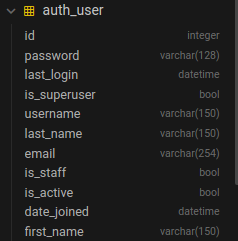
\includegraphics{user}
        \end{figure}

        \begin{figure}[!htb]
            \centering
            \caption{Plant and Info Tables}
            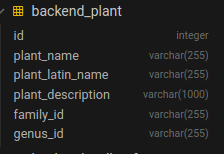
\includegraphics{plant}
            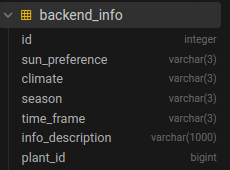
\includegraphics{info2}
        \end{figure}
    
         \begin{figure}[!htb]
            \centering
            \caption{Family, Genus and Edible Tables}
            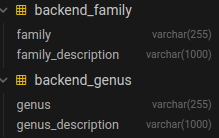
\includegraphics{family-genus}
            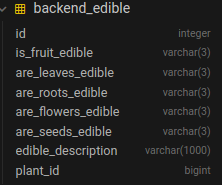
\includegraphics{edible}
        \end{figure}
    
         \begin{figure}[!htb]
            \centering
            \caption{Soil Preference and User Plant}
            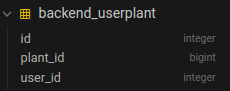
\includegraphics{userplant}
            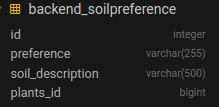
\includegraphics{soil_preference}
        \end{figure}

    
    \newpage
    
	\subsection{Integrating with a Back-end Database}
        Django comes pre setup with sqlite3, a lightweight portable relational database. Django has its own Object Relationship Mapper (ORM). Only after the following can a developer make or showcase any CRUD actions. once a developer has defined their models in the models.py, they need to run \mintinline[bgcolor=bg]{console}|python manage.py makemigrations|, to generate the migration files, Which are Django's way of propagating changes made to your models.
        After Django has finished making the migration files (Which are stored in the appfolder/migrations/ directory, which in our case is backend/migrations/) , you'll need to run \mintinline[bgcolor=bg]{console}|python manage.py migrate|, which creates the necessary tables or changes to your models in the database.
        \\
        
        \begin{wrapfigure}{r}{0.25\textwidth}
            \centering
            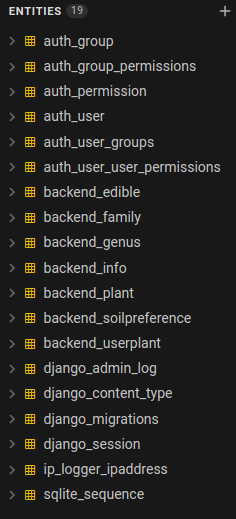
\includegraphics[scale=0.8]{sql1}
            \caption{For clarity here is a Screenshot of the integrated backend database again as shown originally in Fig. 6}
        \end{wrapfigure}
    
        Apart from the code connected with a developer's own custom object as contained in their 'models.py' code, CRUD in Django is handled by the framework without explicit direction from the developer, thus we can test this right away. The only need at this point is that we are logged in as a user using Django's default authentication settings and that the application is functioning.
        \\
        \\
        As mention above Django by default ships with sqlite3 preconfigured, which means our will live in our project folder for the time being. which is in `Plantronics/b.sqlite3'
        \\
        \\
        We can sign into the admin panel and add a 'Plant,' then delete that 'Plant,' to provide two examples of CRUD. To do this step by step, log into the admin panel and follow the steps in :
        \newpage
        \begin{figure}[!htb]
            \centering
            \caption{Once logged in you should be presented by this screen, select the +add option next to plants in the backend list}
            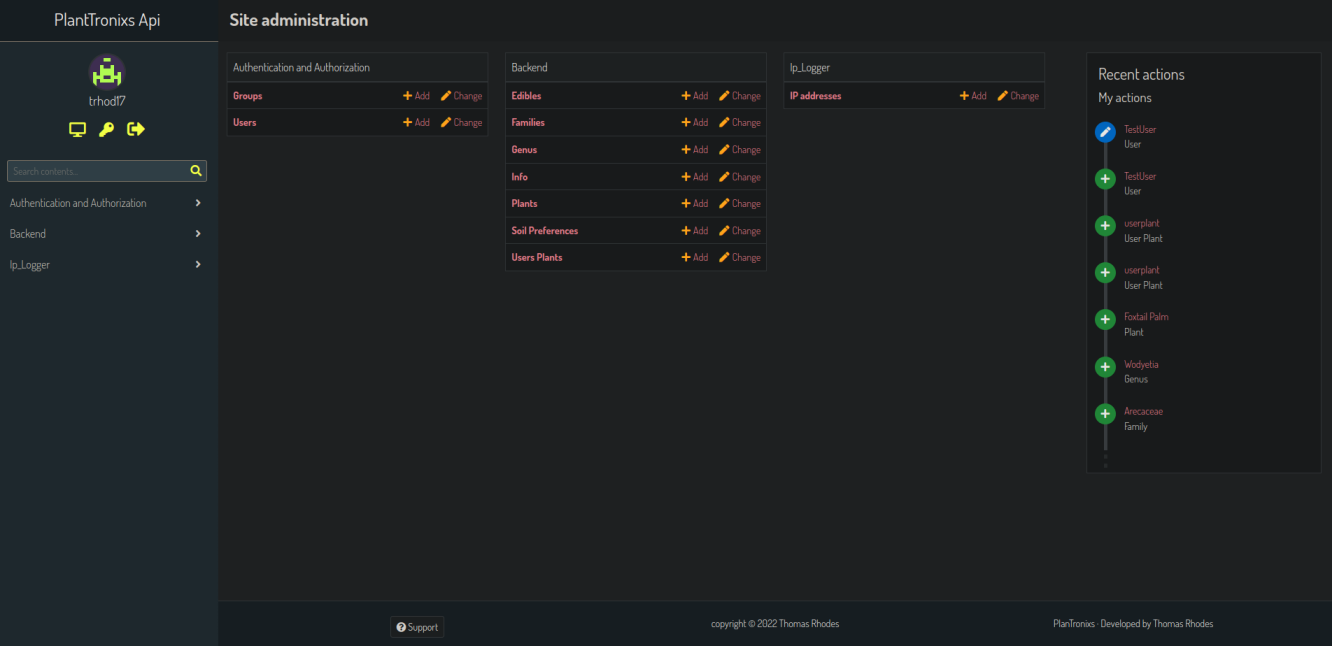
\includegraphics[scale=0.3]{crud1}
        \end{figure}
    
        \begin{figure}[!htb]
            \centering
            \caption{You'll be presented by a screen that looks like this, click the two buttons label `X Remove', we wont be needing those sections. fill out the Plant name, Plant Latin Name, Plant Description (can be left empty), select a family and genus, then select save at the bottom of the screen. Example of filled out form in Fig. 13 below.}
            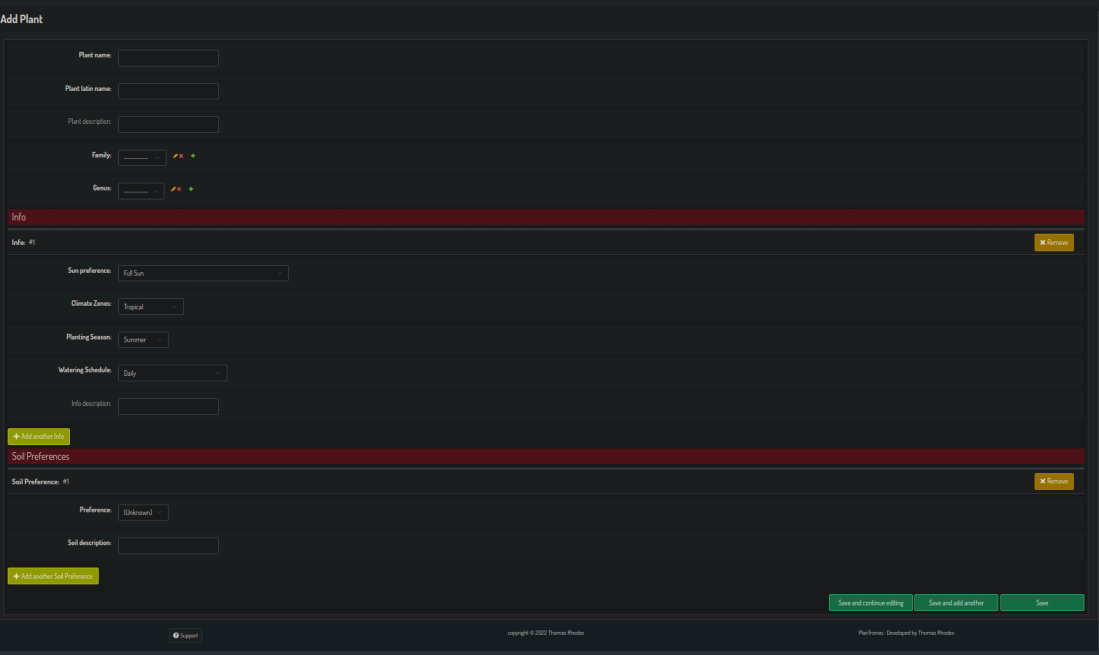
\includegraphics[scale=0.38]{crud2}
        \end{figure}
    
        \begin{figure}
            \centering
            \caption{Example of filled out form}
            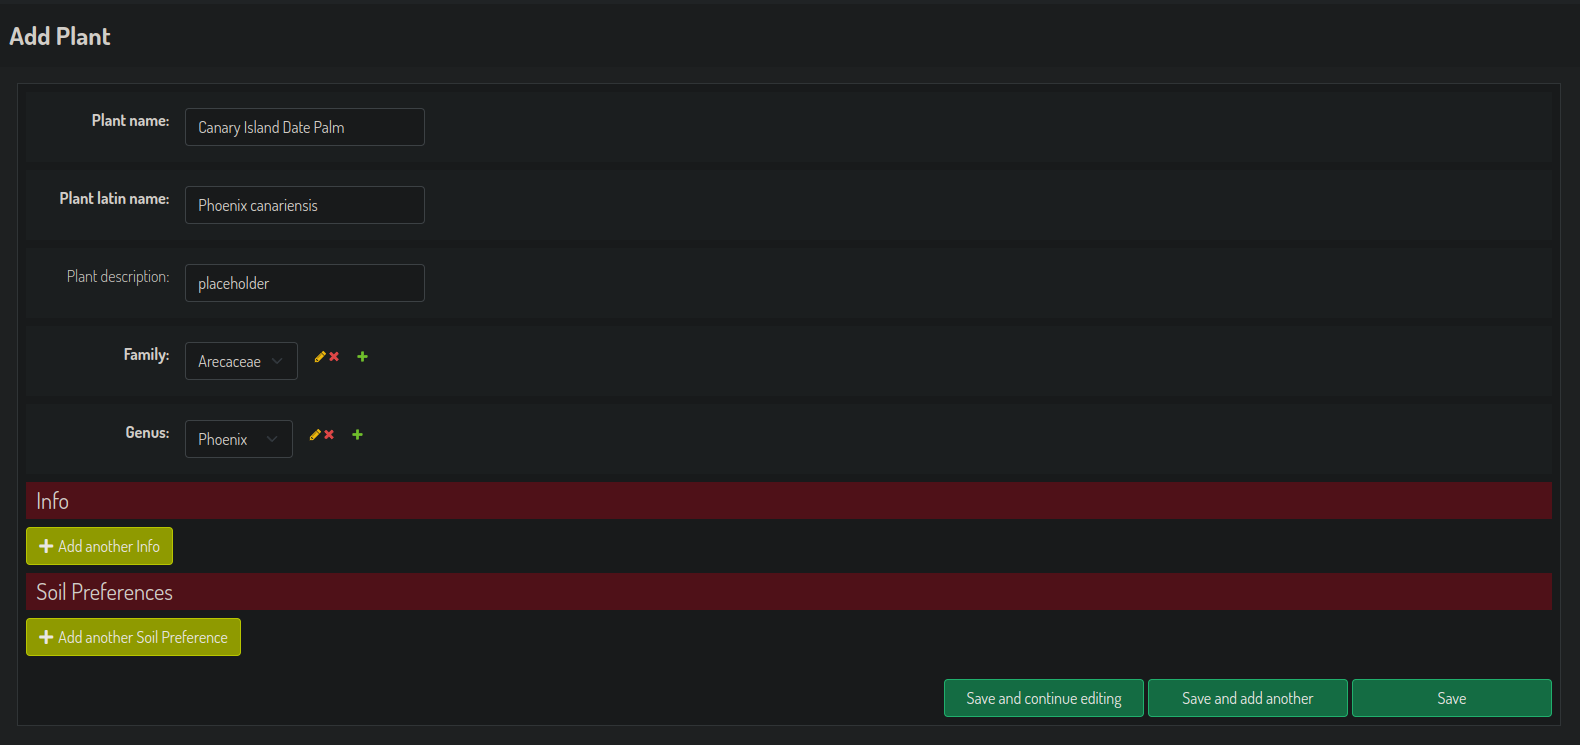
\includegraphics[scale=0.4]{crud3}
        \end{figure}
    
         \begin{figure}
            \centering
            \caption{If it was created successfully it should take you to the following page, Select the plant you created. for this example the plant we created was called the Canary Island Date Palm. Go to Fig. 15}
            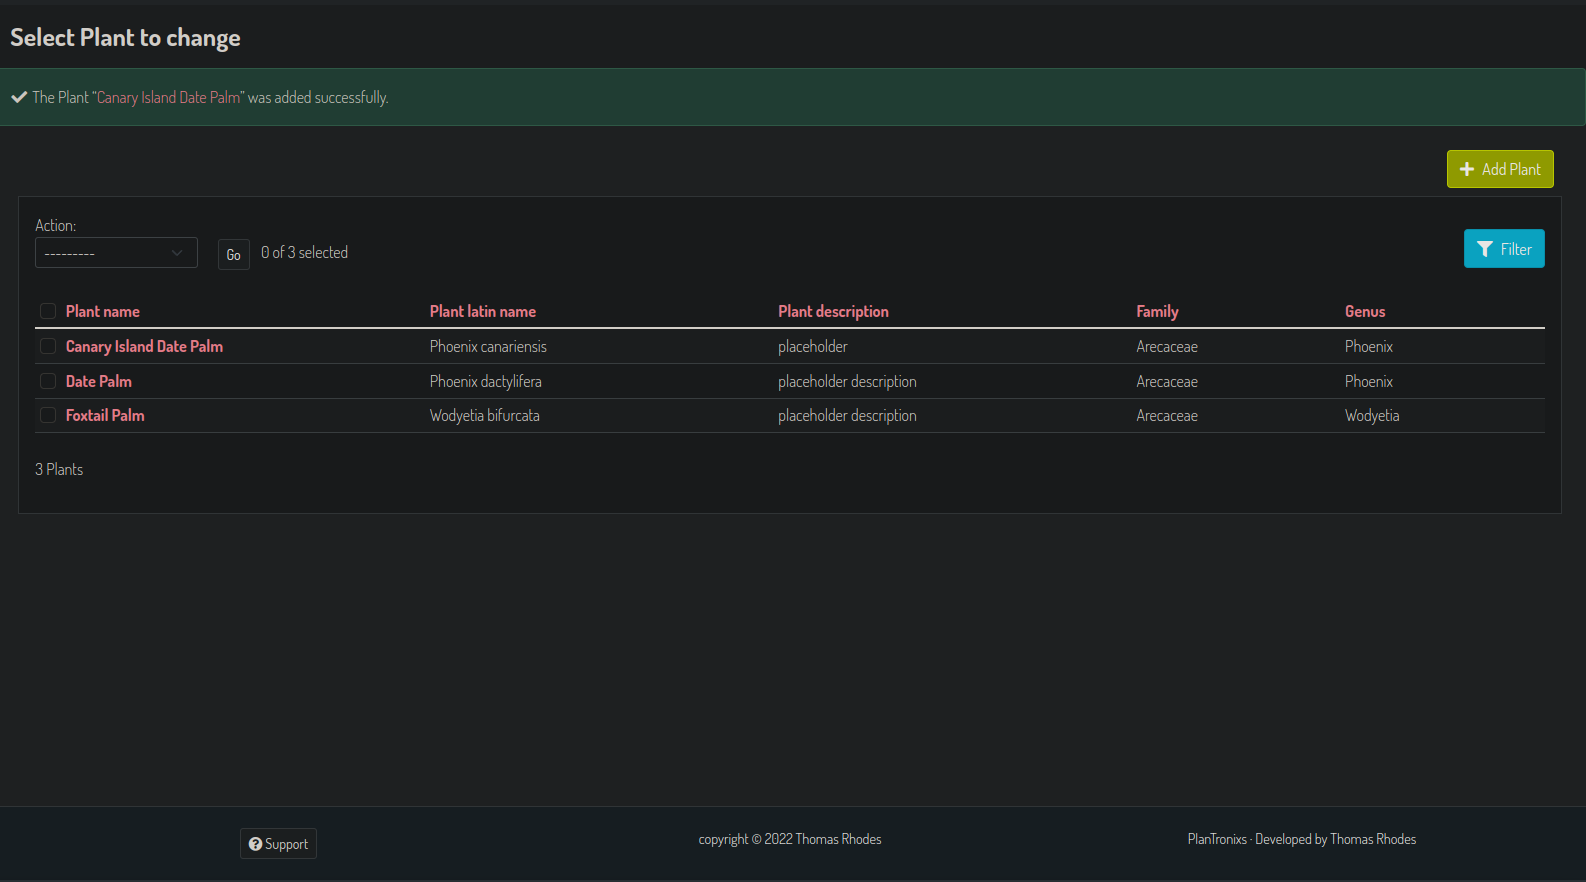
\includegraphics[scale=0.4]{crud4}
        \end{figure}
        
        \begin{figure}
            \centering
            \caption{It should take you to a page like this were you can update, add info or soil preferences, or delete it. In this instance we are going to delete it so click on the delete button in the bottom left corner.}
            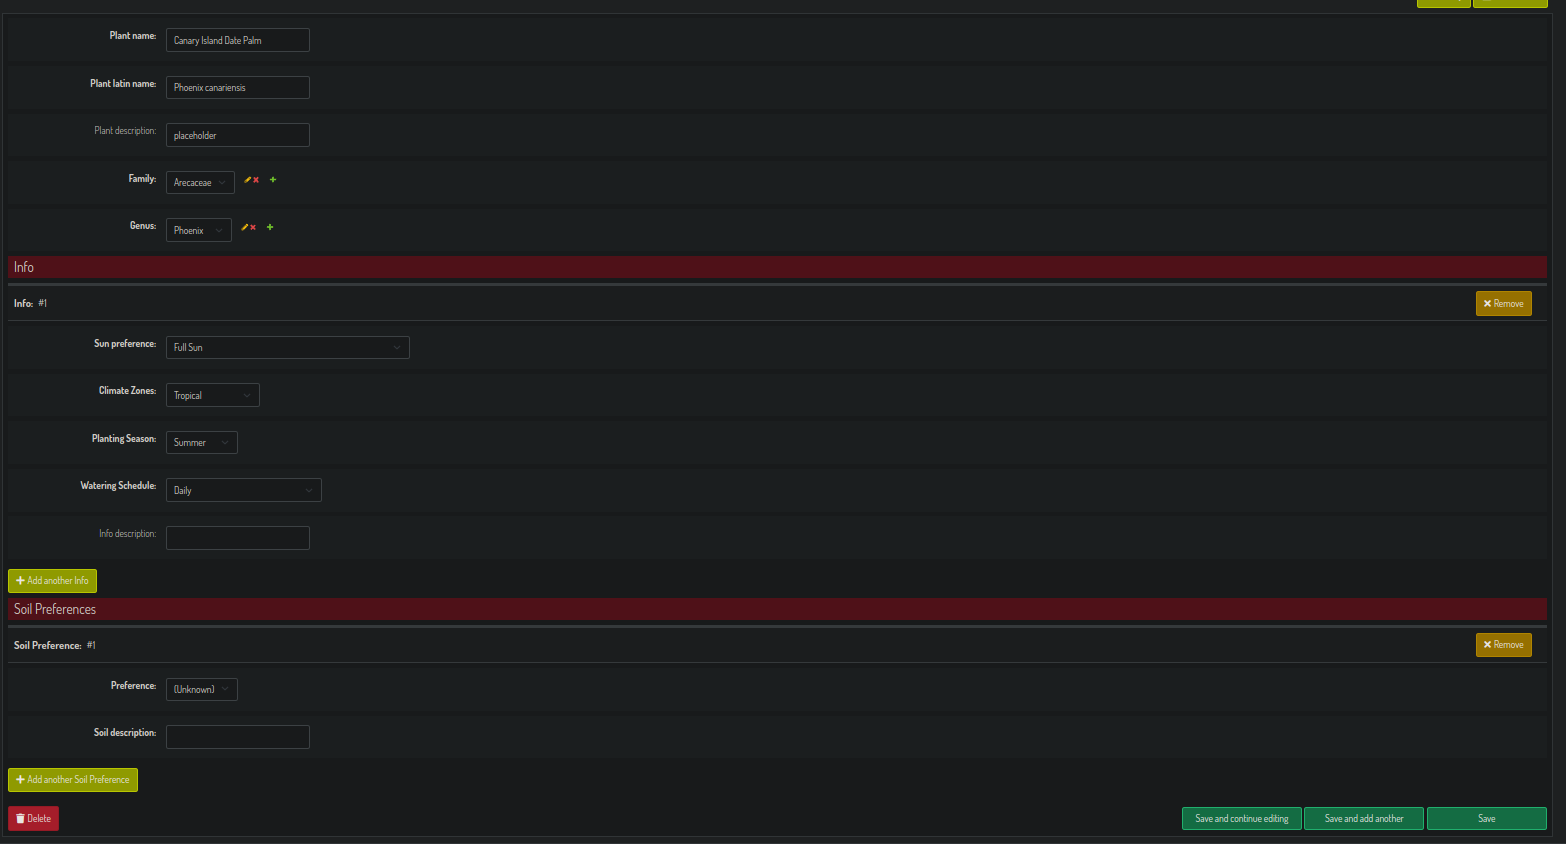
\includegraphics[scale=0.4]{crud5}
        \end{figure}
    
        \begin{figure}
            \centering
            \caption{It will present you with the following confirmation. Press `Yes, I'm Sure' to delete it or `No, Take me back' to cancel this action.}
            \includegraphics[scale=0.4]{crud6}
        \end{figure}
    
        \begin{figure}
            \centering
            \caption{Once its been deleted you'll be taken back to this page and the entry should be deleted successfully.}
            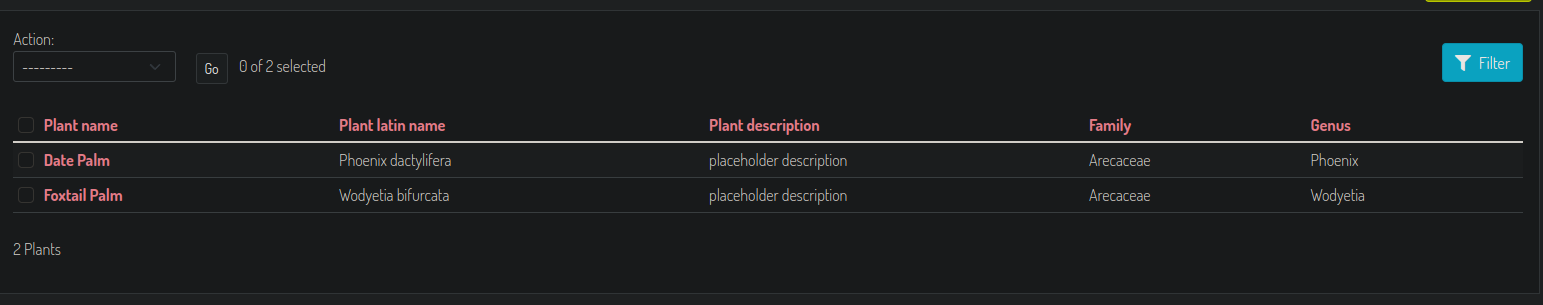
\includegraphics[scale=0.4]{crud7}
        \end{figure}
    
        And thus concludes the integration of a backend database and showcasing 2 crud actions working on said database.
	
	\section{Logging Feature That Records IP, Session, Username, Usertype, Date, and Action for Each Request.}
 
     Logging IP addresses in Django is as easy as running
     \mintinline[bgcolor=bg]{console}|pip install django-ip-logger| 
     and inserting 'ip\_logger' into the installed\_apps list and 'ip\_logger.middleware.LogIPMiddleware' to the
     middleware list in plantronics/settings.py then creating
     and running migrations.
     This plug-in creates a table in the database
     called `ip\_logger\_ipaddress' with four fields: id, ip, init\_visit and last\_visit.  
        
        \begin{figure}[!htb]
            \centering
            \caption{Database Table for IP Logging.}
            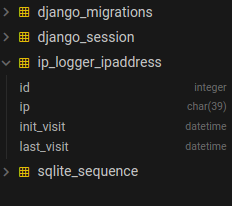
\includegraphics[scale=0.50]{log1}
            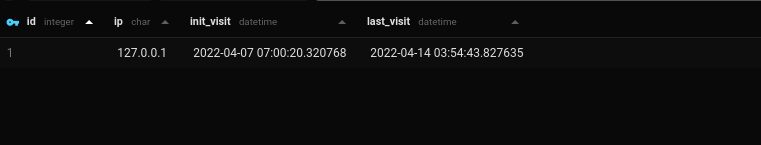
\includegraphics[scale=0.70]{log2}
        \end{figure}  
    
    The justification for logging ip addresses this way as opposed to logging to the console is the persistent nature of databases and deemed necessary to have a separate table for IPs to quickly list all addresses that have made connections to the application. For more information please see the \href{https://pypi.org/project/django-ip-logger/}{about the package django-ip-logger}.
    \\
    \\
    Out of the box, Django logs all requests to the console, for example when directing the browser to \href{http://127.0.0.1:8000/plants/}{http://127.0.0.1:8000/plants/} while the server is running it will log \mintinline[bgcolor=bg]{console}|[14/Apr/2022 15:13:50] "GET /plants/ HTTP/1.1" 200 12345|
    \\
    Django by default logs the Request/Action type, a date-time stamp, and the http status code. The session, username, and user type are not logged, to do this requires some configuration on our part in the settings.py file.
    \\
    \\
    Starting at line 82 and finishing at roughly line 145 in `plantronics/settings.py', is the configuration required to log out the remaining requirements as shown in the screenshot below.
    
    \begin{figure}[!htb]
        \caption{Logging Config}
        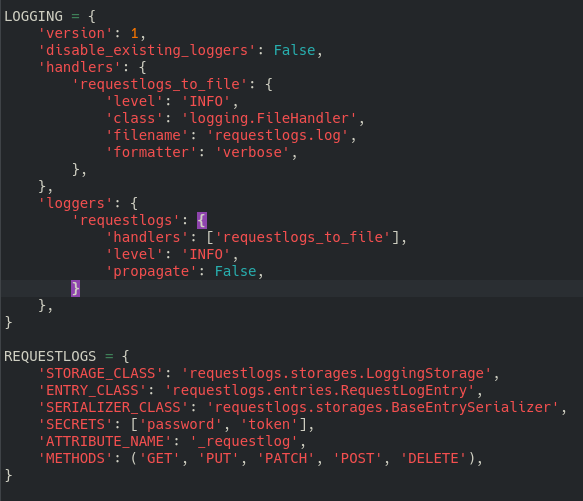
\includegraphics{log3}
    \end{figure}

    A logger in Django is comprised of the logger itself, a handler which decides where to send the data e.g to the console or to a file, filters which further decide which data is to be sent and what is to be kept secret, and formatters which format how the output looks.
    \\
    \\
    The logger in this instance is setup to write the logs to a .log file,
    each log in the file will look something like below:
    
    \begin{minted}[bgcolor=bg]{logtalk}
        requestlogs INFO 2022-04-05 23:39:17,072 storages {'action_name':
        None, 'execution_time': '00:00:00.005267', 'timestamp':
        '2022-04-05T23:39:17.072009Z', 'ip_address': None, 'request':
        OrderedDict([('method', 'GET'), ('full_path',
        '/soilpreference/'), ('data', '{}'), ('query_params',
        '{}'), ('request_headers', '{"HTTP_COOKIE":
        "sessionid=dxur9ryb5i1lqylbla9wf9mqkhzh02w4"}')]),
        'response': OrderedDict([('status_code', 200), ('data',
        '[]')]), 'user': OrderedDict([('id', 2), ('username',
        'test-admin')])} 
    \end{minted}

    Which is only missing the user-type, this is because Django identifies the user-type for each request automatically by comparing `sessionid' values sent in the header of each request. The `sessionid' is a value automatically given to logged in users by Django, which it compares against currently existing `sessionids' to determine if the session is still valid and what permissions the user has. however the user id is logged which means you can search through the users for that id and to find the users type, is\_staff or is\_superuser or permissions/groups.
    
	\section{Rate Limit Session Requests to 1000 per 24 hours per session}

    In most cases rate limiting in Django is as simple as running \mintinline[bgcolor=bg]{console}|pip install django-ratelimit| and configuring it, but in our case because we are using Django rest framework, which has rate limiting built in, there are two simple steps required to set it up
    
    \begin{figure}[!htb]
        \caption{We Create a file called `throttles.py' and add the following code}
        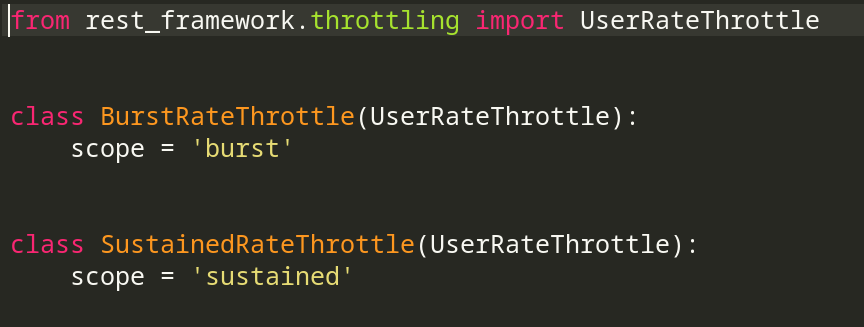
\includegraphics[scale=0.70]{rate1}
    \end{figure}
    
    \begin{figure}[!tb]
        \caption{Then in `settings.py' we add the following to the Django rest framework config}
        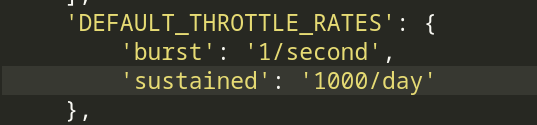
\includegraphics{rate2}
    \end{figure}
    \newpage
    
    To make sure its works, we can test by launching the server and reloading any page as fast as possible, in the console you should see messages like this 
    \begin{minted}[bgcolor=bg]{logtalk}
    Too Many Requests: /
    [16/Apr/2022 02:16:57] "GET / HTTP/1.1" 429 5413
    \end{minted}
    
    and in the sake of our sanity when it comes to testing the sustained rate limiting we will change it to 5 per day rather than 1000 and you should see a message similar to the one above and get a message on the webpage similar to below:
    \\
    \begin{figure}[!htb]
        \caption{Rate Limited}
        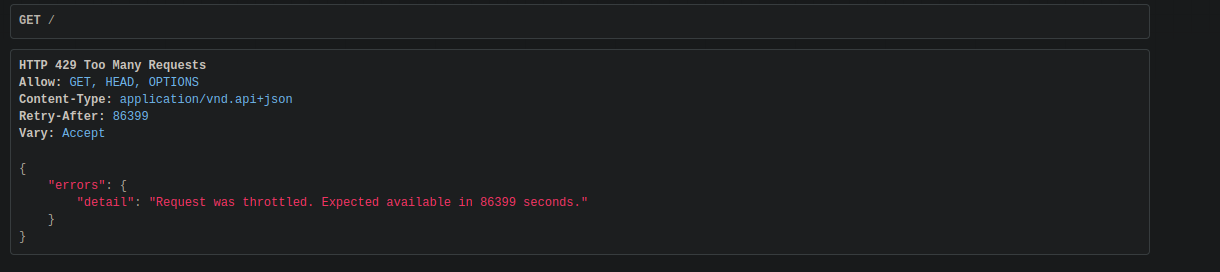
\includegraphics[scale=0.50]{rate3}
    \end{figure}
    \newpage
	\section{Domain Locking Web Service to Whitelisted Referrers}
    To enable and setup whitelisting in Django requires the following steps:
    
    
    \begin{figure}[!htb]
        \caption{First create a list in settings.py called REST\_SAFE\_LIST\_IPS and add whatever ips you want to it:}
        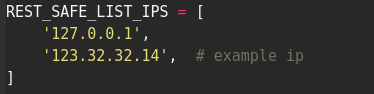
\includegraphics[scale=0.50]{whitelist1}
    \end{figure}
    
    \begin{figure}[!htb]
        \caption{In the same directory as the settings.py file create a new file called safelistpermissions.py and add in the following:}
       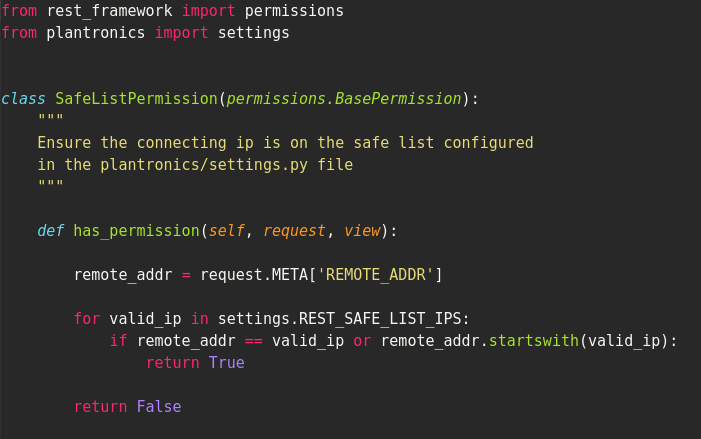
\includegraphics[scale=0.50]{whitelist2}
    \end{figure}
    
        The first two lines import the Django Rest Frameworks permission function and import the settings.py file, this needs to be done provide rest\_framework\_permissions.BasePermission a custom subclass.
        
        \begin{figure}[!htb]
            \caption{At the bottom of the Django rest framework array in settings.py add in the following:}
            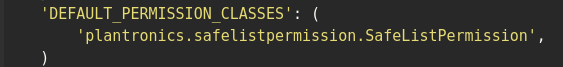
\includegraphics[scale=0.50]{whitelist3}
        \end{figure}
        \pagebreak
        SafelistPermission is used to allow certain IPs defined in the settings.py::REST\_SAFE\_LIST\_IPS access to the service.
        \\
 
        If we comment out all of the IPs in REST\_SAFE\_LIST\_IPS and try to connect to the web service well get the following message:
    \newline
    \begin{figure}[!htb]
       \caption{It will force a false value and deny you access to the service}
       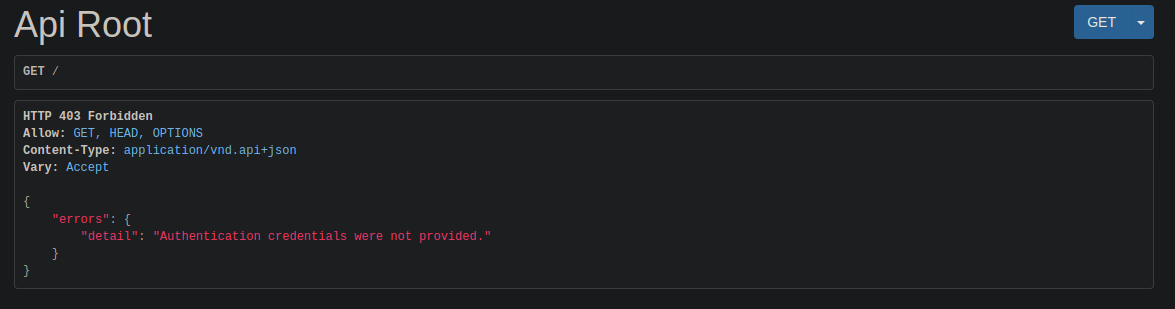
\includegraphics[scale=0.50]{whitelist4}
    \end{figure}

    \pagebreak
	\part{Code Structure}
    \begin{spacing}{4}
    \end{spacing}
    
	\section{Custom Written Database Option}
    In Django user defined entities/database objects are created in the `models.py' file, Django uses a custom ORM for writing these objects, which comes preconfigured to translate what we see below into sqlite3 which is sent to and run on the database to setup or update the database tables/rows/columns/etc.
    
     \begin{figure}[!htb]
        \caption{models.py}
        \centering
        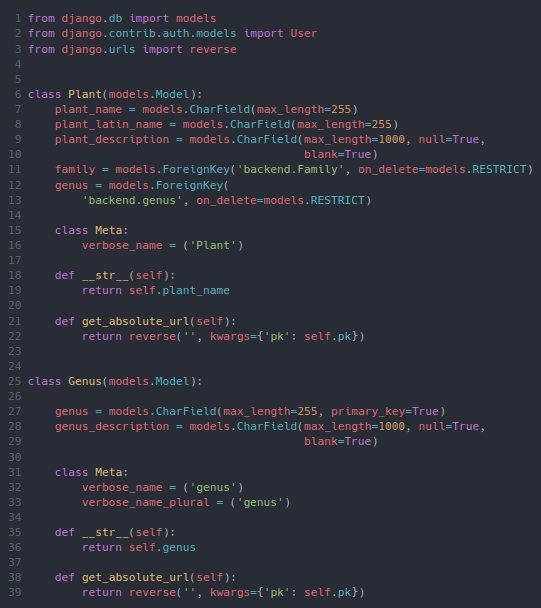
\includegraphics[scale=0.8]{models1}
    \end{figure}


    Django also has official support for PostgreSQL, MariaDB, MySQL, Oracle SQL, and Django also has many third party backends or engines as there sometimes called for using other databases.
    \\
    \\
    After saving our models.py and running \mintinline[bgcolor=bg]{console}|python manage.py makemigrations|
    which creates a migration file with the changes the need to be made to either create or update the database,
    then \mintinline[bgcolor=bg]{console}|python manage.py migrate|,
    which creates and updates all the required tables/columns/etc. in your database.
   
    
    \begin{figure}[!htb]
        \caption{As shown here is the associated SQL for creating the SQLite 3 database for this project}.
        \centering
        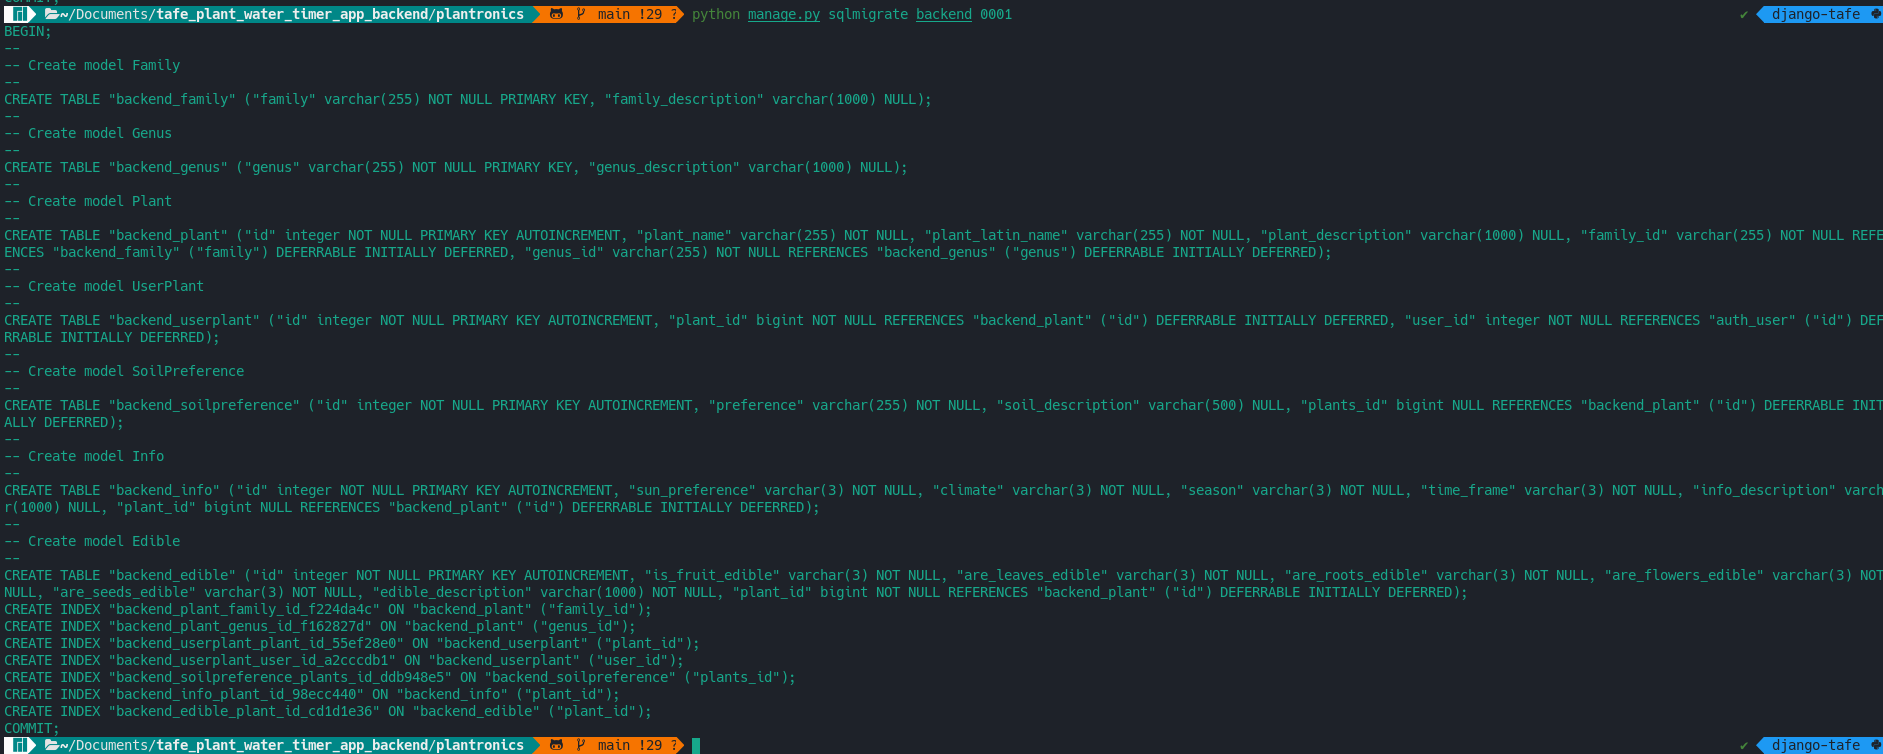
\includegraphics[scale=0.35]{sqlb1}
    \end{figure}

     \newpage

    \section{use request, response and session objects rather then their superglobals}
    
    Unlike languages like PHP, Python and by extension Django have no such thing as a SuperGlobal, mainly because the Python devs dont want to support the use of this type of functionality, However global variables do exist, which are variables written outside of functions and can be called in other files by importing them e.g \mintinline[bgcolor=bg]{console}|from main import x|, which import the variable x from the file main.py.
    \\
    \\
    In Django request, response and session objects are handled by serializers, views, and django.auth.contrib which is its built-in authentication backend, transaction requests are handled in views.py.
    
     \begin{figure}[!htb]
        \centering
        \caption{Views.py 1/3}
        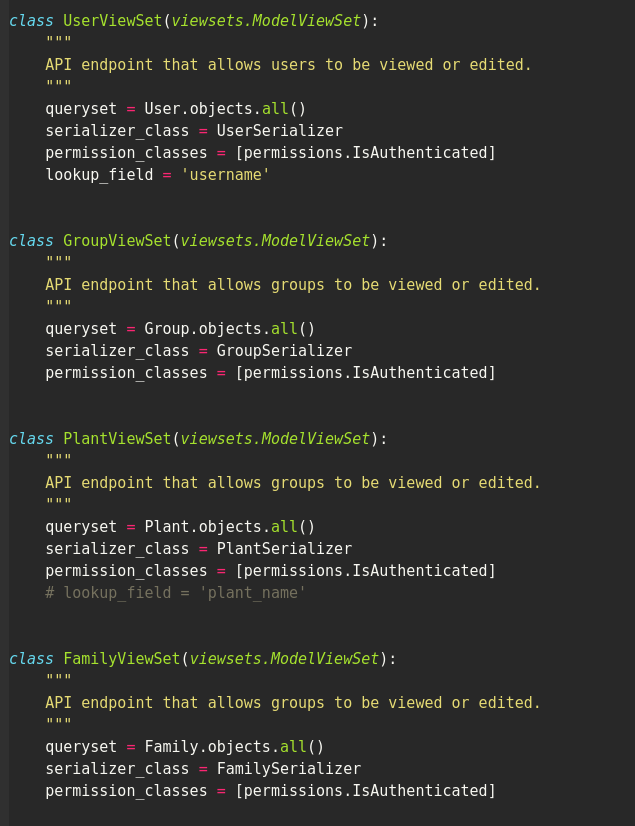
\includegraphics[scale=0.50]{views1}
    \end{figure}

     \begin{figure}[!htb]
        \centering
        \caption{Views.py 2/3}
        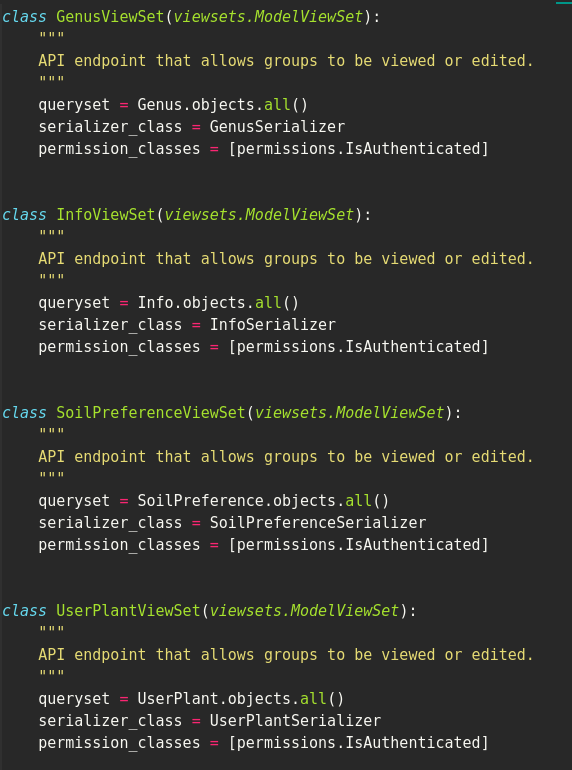
\includegraphics[scale=0.50]{views2}
    \end{figure}

     \begin{figure}[!htb]
        \centering
        \caption{Views.py 3/3}
        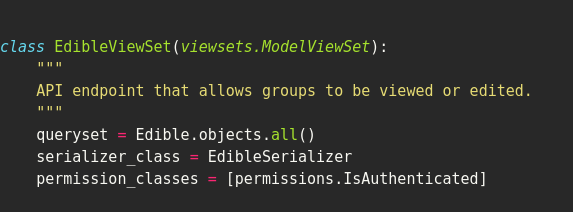
\includegraphics[scale=0.50]{views3}
    \end{figure}
   
  \newpage
    
      
    \section{Use at least three http response codes including 200}
    
    Django is designed to respond to all requests with all the http codes logged to the console, below are some screens of response logged to the console by Django:
    
    \begin{figure}[!htb]
        \centering
        \caption{response codes}
        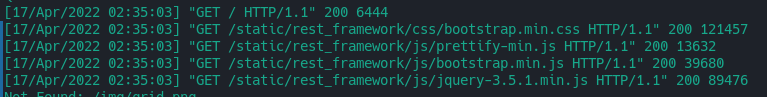
\includegraphics[scale=0.8]{response1}
    \end{figure}

      \begin{figure}[!htb]
         \centering
         \caption{response codes}
         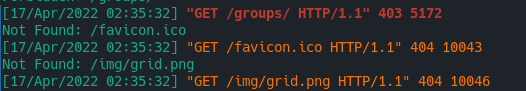
\includegraphics{response2}
     \end{figure}

     \begin{figure}[!htb]
        \centering
        \caption{response codes}
        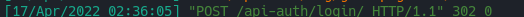
\includegraphics{response3}
    \end{figure}

     \begin{figure}[!htb]
        \centering
        \caption{response codes}
        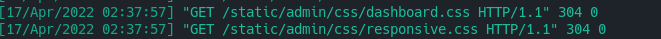
\includegraphics{response4}
    \end{figure}

     \begin{figure}[!htb]
        \centering
        \caption{response codes}
        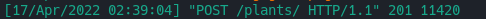
\includegraphics{response5}
    \end{figure}
    
    
    \newpage
    
    \section{Response Data}
    
    \subsection{Validation of GET and POST data before it is serialized or processed by an object}
    
     \subsubsection{POST Requests}
      POST data such as Users, Plants, Family, Genus, etc,
      the data must contain all fields present in the model including fields which are not required which can be left empty, for example Family consists of 2 user defined fields, family and family\_description, family is required and the post request will fail if its left empty by family\_description isn't so it can be left empty when submitting the request without any consequences.
      both of the aforementioned user defined fields are both varchar fields if the POST request tries to submit data that doesn't conform to the fields format the request will not be accepted with a response stating malformed object data or something similar. some data can only by changed or updated by users who have either is\_staff or is\_superuser, which is defined in Django's user model as booleans, set to True. 
      
     \subsubsection{GET Requests}
     
     Depending on what your trying to GET, GET requests are handled by various different means, if you trying to access the admin panel your request will be denied unless you login or are logged in as a staff user or superuser which is handled by Django's inbuilt auth system, other pages such as the Django Rest Api pages are by default accessibly by anyone but are configured in this instance to only allow registered users access to these pages.
    
    \subsubsection{Additional Validation}
    
    Additional validation is handled by various functions of Django and Django Rest Framework which are listed below:
    
    \begin{minted}[bgcolor=bg]{console}
        'rest_framework_json_api.filters.QueryParameterValidationFilter'
        'django.contrib.auth.password_validation.UserAttributeSimilarityValidator' 
        'django.contrib.auth.password_validation.MinimumLengthValidator'
        'django.contrib.auth.password_validation.CommonPasswordValidator'
        'django.contrib.auth.password_validation.NumericPasswordValidator'
        'django.contrib.auth.middleware.AuthenticationMiddleware'
        'django.contrib.sessions.middleware.SessionMiddleware'
        'django.middleware.security.SecurityMiddleware'
    \end{minted}

    \subsection{Response Format}
        Into order to turn our app into a JSON churning machine, we must make some changes to the Django Rest Framework Config in settings.py as shown below:
        
        
        \begin{figure}[!htb]
            \centering
            \caption{Django Rest Framework Config}
            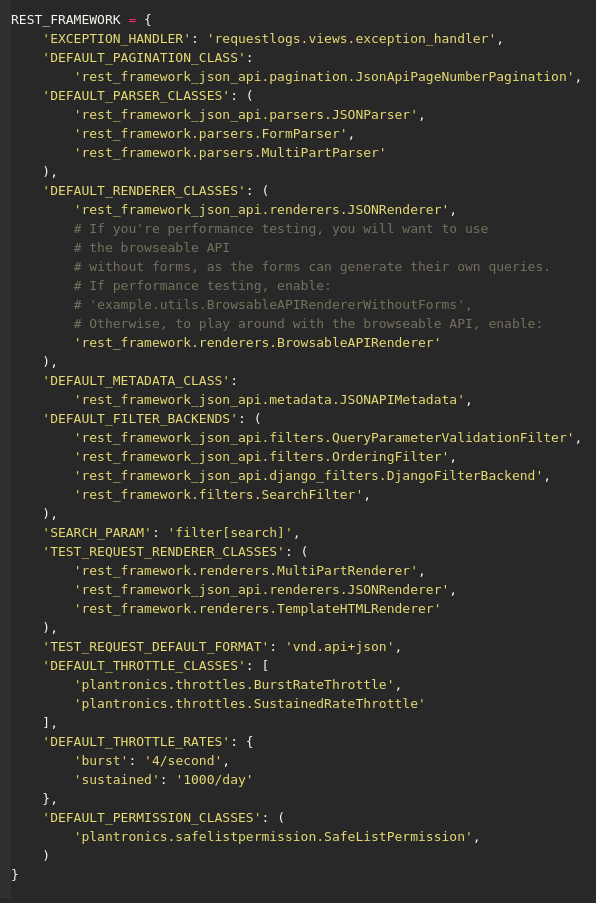
\includegraphics[scale=0.50]{format1}
        \end{figure}
    
    once we have done that going to any of the api pages will present us with the following.
    
    
    \begin{figure}[!htb]
        \centering
        \caption{Family Api Page}
        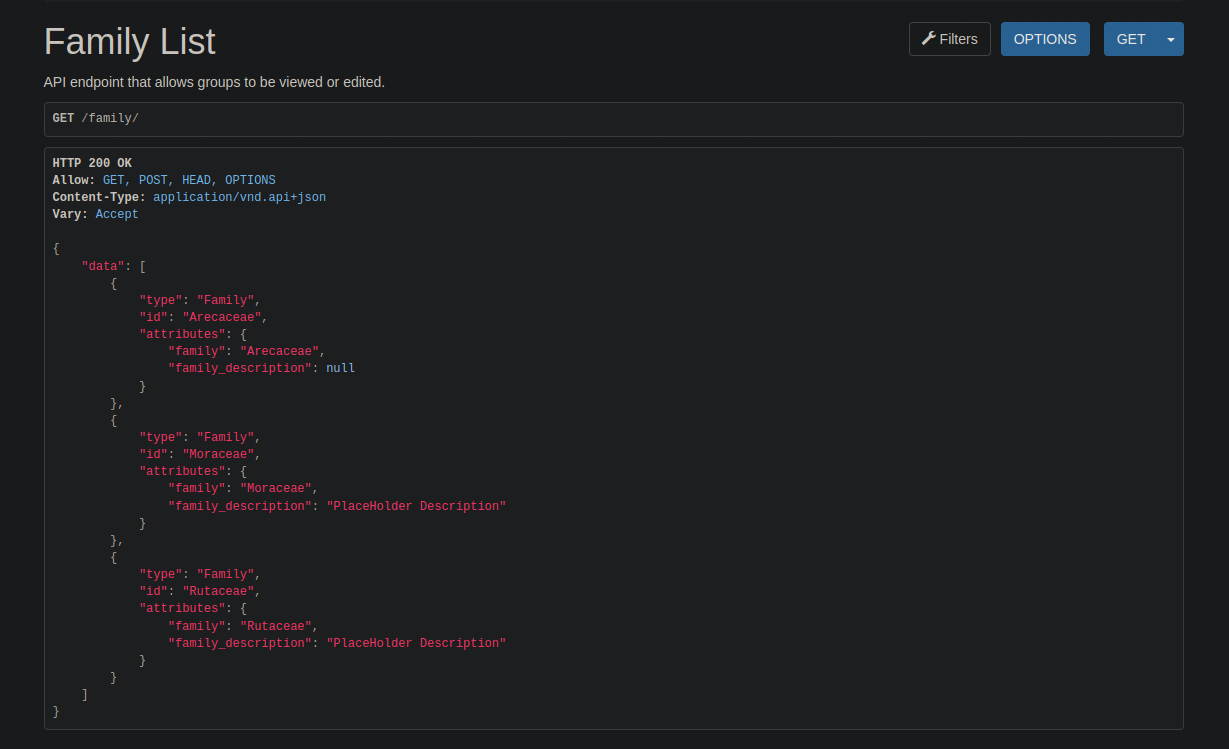
\includegraphics[scale=0.50]{format2}
    \end{figure}

    In the above the content-type is automatically set as vnd.api+json, however as this page will never be seen by users we must test this in the same way a user will interacted with it, well closer to how a user will interact with it anyway, by using a piece of software known as Postman to send a get requests to the api.
    
    
    \begin{figure}[!htb]
        \centering
        \caption{Get request, to the home page}
        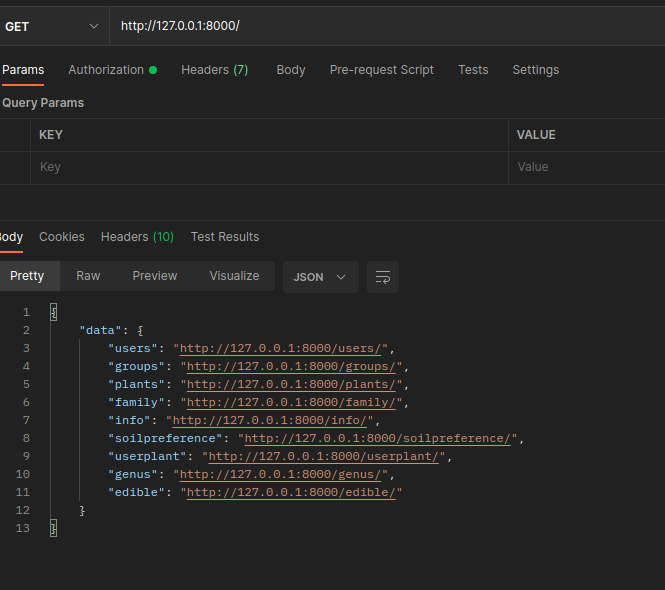
\includegraphics[scale=0.50]{format3}
    \end{figure}

    
    \begin{figure}[!htb]
        \centering
        \caption{Get request, to the plant page}
        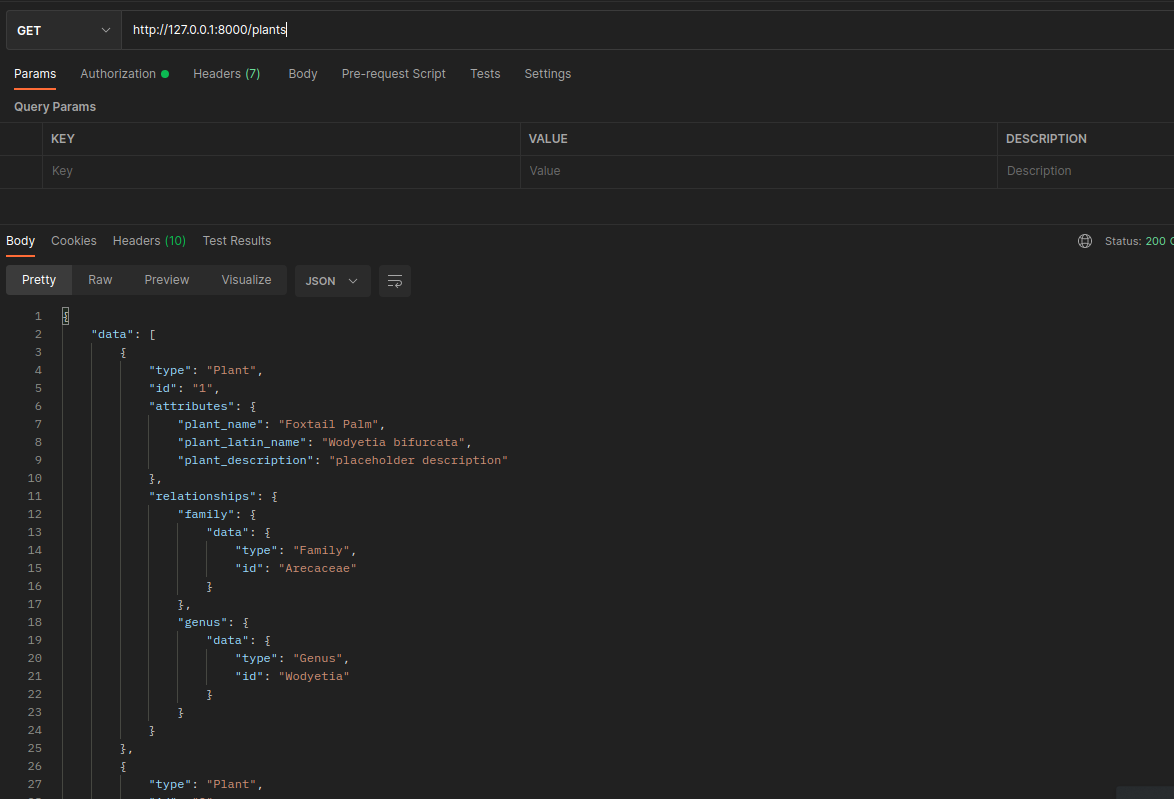
\includegraphics[scale=0.50]{format4}
    \end{figure}

    
    \begin{figure}[!htb]
        \centering
        \caption{Get request, to the plant/1 to get the first plant}
        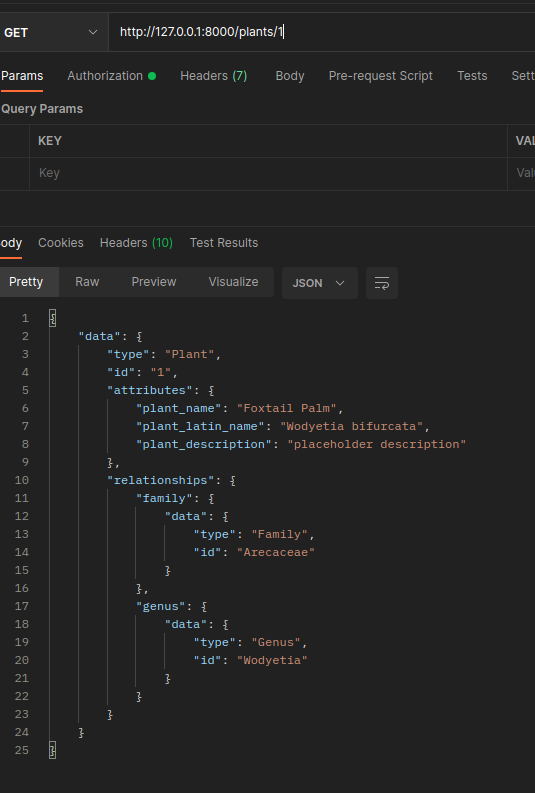
\includegraphics[scale=0.50]{format5}
    \end{figure}

    As is displayed in the previous images the data is displayed in the JSON format, this format will be used by the frontend and server to send and receive data to/from each other.
    
    \newpage
    
    \part{Code Comments}
    \begin{spacing}{4}
    \end{spacing}
   
    \section{Explain why you created the database and session objects in that particular location}
    The database models were instantiated in models.py as is defined/required by Django, models.py is located in the backend folder. The reason for this is that Django follows the MVC folder structure, and Django likes to separate the main program which in this case is plantronics and its child applications which in this case is backend. Django prefers and insists developers create new apps rather then working in the main program directory because it allows for better readability and separation of sometimes fundamentally different parts of an program.
    \\
    \\
    The models.py file in our application is where Django requires we build our database objects, The reason for this is that Django is preconfigured to use code from certain preconfigured locations such as models.py. Another maybe better way to explain this is that Django is a semi opinionated framework, which means it assumes some things like where are database objects are stored, but some things like whats shown to the user is left up to us. This is true for the database type as well, because by default Django is setup to use SQLite which makes sense in development and would most likely be changed in later closer to deployment.
    \\
    \\
    Sessions and Session objects are handled by a middleware application called 'django.contrib.sessionsMIDDLEWARE' which needs to be Enabled to work, the session objects are stored in a table in the database called django\_session.
    
    \section{Explain the arithmetic behind one of your rate-limiting codes}

    \begin{figure}[!htb]
        \centering
        \caption{Our Rate Limiters}
        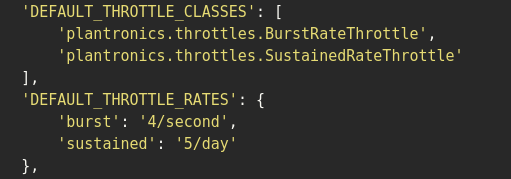
\includegraphics[scale=0.70]{ratelimit1}
    \end{figure}
    
    We technically have two rate limiters, burst and sustained, burst allows each unique request origin to make 1 request for every second passed, which means for each connected ip address there is a counter and when the counter is greater then one in a give second, any additional requests are from that ip are rejected until the block is lifted for that ip which usually happens after one to two seconds.
    \\
    \\
    For sustained rate limiting, in the code is specified as 1000/day, meaning for every unique request origin no more then 1000 requests can be made in a twenty four hour period as measured in Universal Basic Time (UTC), so once a unique address as surpassed that limit it will be blocked for one UTC day before being allow to send more requests.
    \\
    \\
    Simply put once a IP address surpasses the defined limit for which each request made is recorded, they will no longer be able to make any more request until there cool down period is over.  
    
    \section{Note where you're testing to see if a session already exists and what you'll do if it does}
    
    In Django sessions are stored in the database in a table called  django\_sessions, in Django SESSION\_EXPIRE\_AT\_BROWSER\_CLOSE is set to false, which means Django will store the sessions in the database until they and the cookie saved on the client expire, every time a unique request its made whether from a new browser or with a different header or set of headers it will create a new session. If the header of the browser connecting to the site contains the session cookie it will resume interacting with the site as a persistent user as long as the cookie has not expired and self destructed on either end determined by SESSION\_COOKIE\_AGE, this is handled by Django's session middleware.
    \\
    \\
    For further information refer to: \href{https://github.com/django/django/blob/main/django/middleware/csrf.py}{Django csrf.py github}.
    
    \section{Describe the code structure that verifies all GET/POST structures}
    Before each and every GET and Post request is processed, a UID or unique identifier is either sent in the request header or a new UID is set which itself is a cookie, which is stored in Django's Auth table and the users browsers. This cookie is automatically compare by Django's authentication middleware, which is used to track user interactions and validating which user has done what.
    
    Each field has a associated data type and max length, for example the info table has a field called sun\_preference which has a max length of 3 characters meaning it can only accept a string of 3 or less characters, the characters can be alphabetical, numerical or other special characters as long as its a string, the purpose of the 3 character limit is that, its purpose is to accept a key which maps to a choice provided in the model, if someone trys to post a new info data with the sun\_preference set to a invalid choice the post request would be denied.
    

    \begin{figure}[!htb]
        \centering
        \caption{Serializers}
        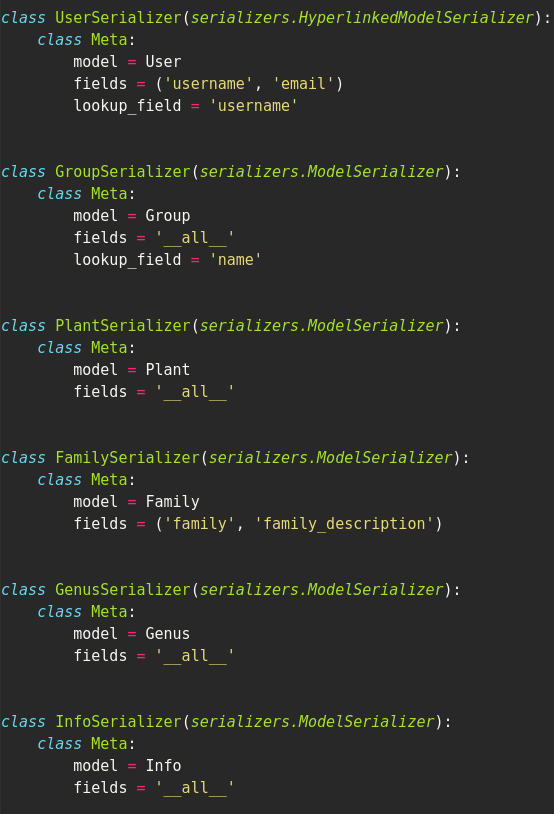
\includegraphics[scale=0.40]{serializers1}
    \end{figure}

     \begin{figure}[!htb]
        \centering
        \caption{Serializers}
        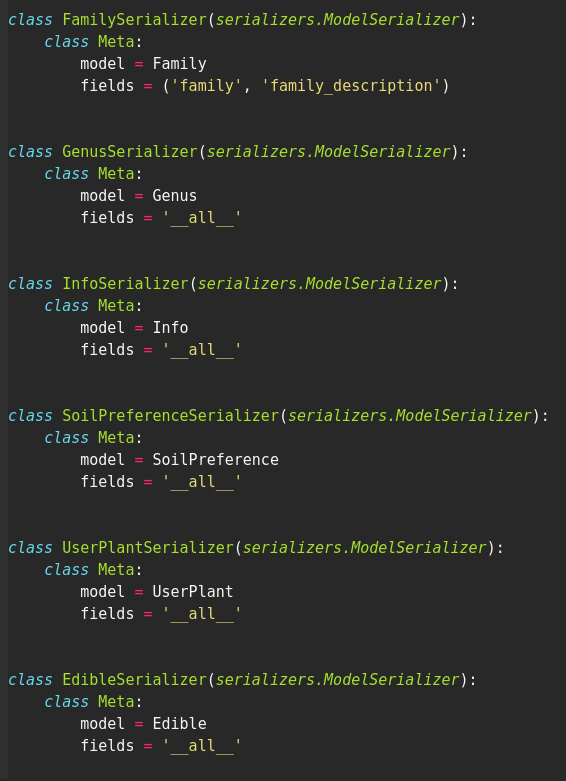
\includegraphics[scale=0.40]{serializers2}
    \end{figure}
    
    A serializers role is to specify the metadata for what a entity is and fields associate with it so that the data received may be translated from JSON to Python code and vice versa, serializers also allow developers to set a list of fields which are contained inside manually, but Django has the option '\_\_all\_\_' which is used to display all fields in a get request, but for example if you were to make a GET request for info with soilpreference of any  which dosent exist in info, it will return a malformed json error, which also provides another layer of security and validation.
    \\
    \\
    Django's default auth model handles the necessary checks to determine if the user has the correct privileges in order to do certain actions. 
    \newpage
   
    \section{Write a README file that explains how to setup and configure this service}
    See Attached README.pdf in the same folder as this documentation
    
    \section{As part of unit testing, create a test script that interacts with the web service to test all known GET and POST requests.}
    
     There are eight total tests with each test containing three subtests, one post test, one get all test, and one get specific test. Which in total comes to 24 tests, in order to run all those test without getting rate limited there are two options, option 1 is to increase the burst rate limit to 4 or more per second, the second option which i chose to go with uses the python time library to wait around 0.4 seconds before preceding to the next test.

     \begin{center}
     \title{Test Cases}
     \begin{figure}[!htb]
         \centering
         \caption{Test Cases 1/3}
         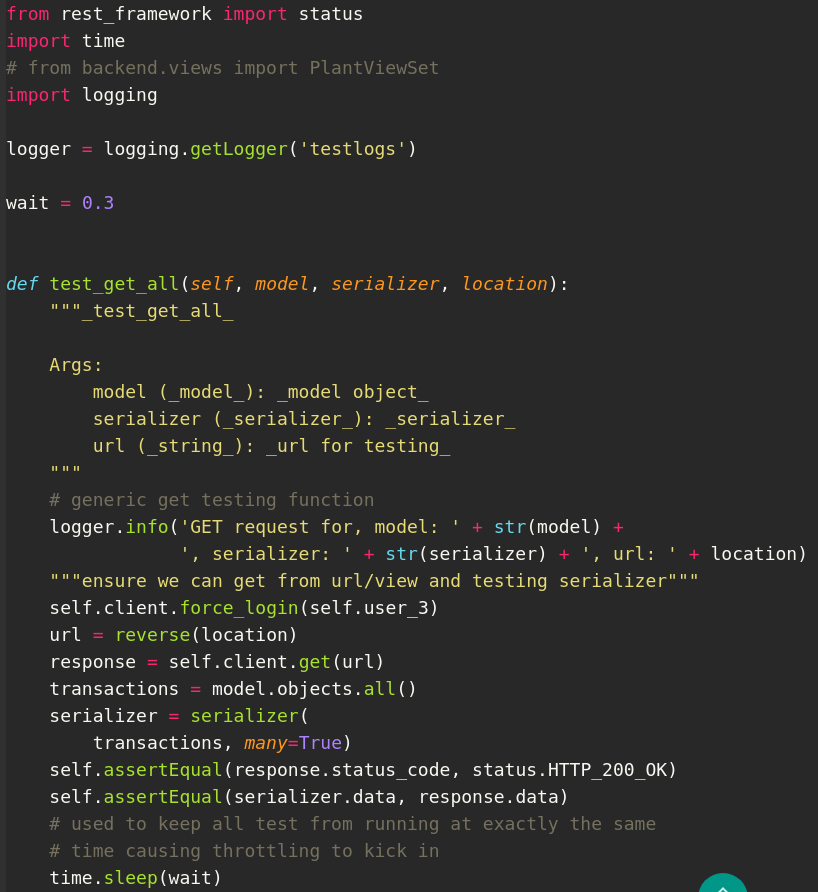
\includegraphics[scale=0.50]{testcase1}
     \end{figure}

      \begin{figure}[!htb]
          \centering
          \caption{Test Cases 3/3}
          \includegraphics[scale=0.50]{testcase3}
      \end{figure}
      
      \begin{figure}[!htb]
          \centering
          \caption{Test Cases 3/3}
          \includegraphics[scale=0.50]{testcase3}
      \end{figure}
      \newpage
      \title{Tests}
      \begin{figure}[!htb]
          \centering
          \caption{Tests 1/5}
          \includegraphics[scale=0.50]{test1}
      \end{figure}
  
       \begin{figure}[!htb]
           \centering
           \caption{Tests 2/5}
           \includegraphics[scale=0.50]{tests2}
       \end{figure}
       
       \begin{figure}[!htb]
           \centering
           \caption{Tests 3/5}
           \includegraphics[scale=0.50]{test3}
       \end{figure}
       
       \begin{figure}[!htb]
           \centering
           \caption{Tests 4/5}
           \includegraphics[scale=0.50]{tests4}
       \end{figure}
       
       \begin{figure}[!htb]
           \centering
           \caption{Tests 5/5}
           \includegraphics[scale=0.50]{tests5}
       \end{figure}
       \end{center}
    
	
\end{document}
